\documentclass[12pt, a4paper]{article}

\usepackage[T1]{fontenc}
\usepackage{graphicx}
\usepackage{hyperref}
\usepackage[brazil]{babel}
\usepackage{geometry}
\usepackage{color}
\usepackage{pythonhighlight}
\usepackage[utf8]{inputenc}
\usepackage{indentfirst}
\lstset{
	numbers=left,
}

\geometry{
	a4paper,
	left=30mm,
	right=20mm,
	top=30mm,
	bottom=20mm
}

\title{
    \textbf{IESB} \\
    \large Big Data e Inteligência Analítica \\
    \vspace{10cm}
    \textbf{Projeto Integrador em Big Data e Inteligência Analítica}
    \author{Lucas Siqueira Rodrigues}
}


\begin{document}

\begin{titlepage}
    \maketitle
    \begin{center}
        \vspace{\fill}
        Brasília - DF \\
        Junho de 2025
    \end{center}
\end{titlepage}


\section{Obtenção da base de dados}
\subsection{Introdução}
O trabalho tem como objetivo explorar os dados públicos disponibilizados pela Câmara dos Deputados para analisar e compreender os gastos realizados pelos parlamentares. Para isso, os dados serão obtidos por meio do portal dos dados abertos da câmara\cite{dados_abertos}, armazenados em um banco de dados relacional na nuvem e, posteriormente, analisados.

\subsection{Motivação}
A transparência pública é essencial para garantir a confiança da população nas instituições governamentais. Esse projeto busca realizar um ciclo completo de extração, transformação, armazenamento e análise dos dados de gastos públicos. Além disso, ao construir dashboards dinâmicos espera-se fornecer ferramentas que possam auxiliar na identificação de possíveis irregularidades e na fiscalização das despesas parlamentares.


\subsection{Script e Banco de Dados}
Para o ano de 2022, a obtenção dos dados por meio da API\cite{dados_abertos} retornou apenas 32 registros.

\begin{python}
import io
import json
import zipfile

import httpx
from tqdm import tqdm

class CamaraAPI:
	def __init__(self) -> None:
		self.base_url = "https://dadosabertos.camara.leg.br/api/v2"
	
	def request(self, endpoint: str) -> dict:
		response = httpx.get(f"{self.base_url}/{endpoint}")
		return response.json()
	
	def get_deputados(self) -> dict:
		return self.request("deputados").get("dados", {})
	
	def get_despesas(self, id_: int, year: int = 2022) -> dict:
		return self.request(f"deputados/{id_}/despesas?ano={year}")

despesas = []

api = CamaraAPI()

deputados = api.get_deputados()
for deputado in tqdm(deputados):
	id_ = deputado["id"]
	despesas_deputado = api.get_despesas(id_=id_, year=2022)
	despesas.extend(despesas_deputado["dados"])
print(len(despesas))
\end{python}


\begin{figure}[h]
    \centering
    % Substitua 'imagem1.png' pelo nome do seu arquivo de imagem
    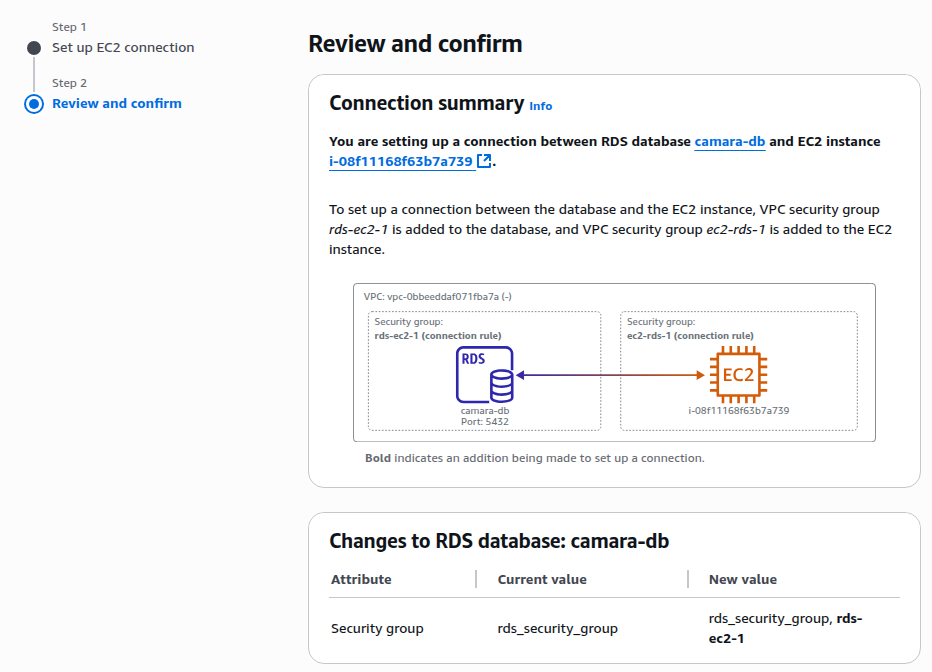
\includegraphics[width=0.8\textwidth]{assets/1.png} 
    \caption{Coleta de dados por meio da API para o ano de 2022.}
    \label{fig:api_2022}
\end{figure}

Por isso, apenas para esse ano a coleta de dados foi por meio de um arquivo no formato JSON, que também é fornecido no portal de dados abertos da câmara por meio da aba “Arquivos”.

\begin{figure}[h]
    \centering
    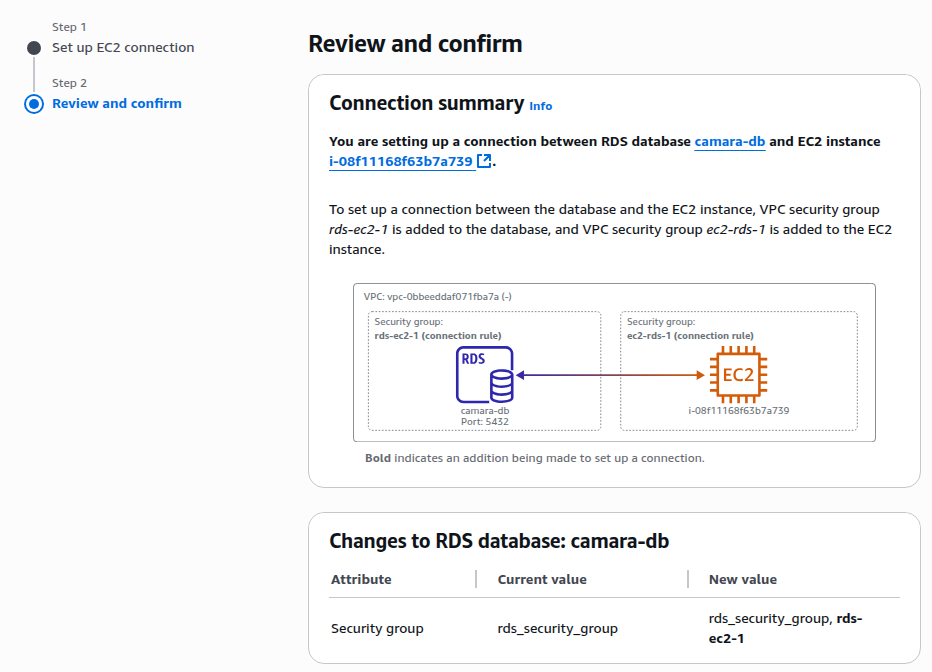
\includegraphics[width=0.8\textwidth]{assets/1.png}
    \caption{Coleta de dados por meio do arquivo.}
    \label{fig:arquivo_json}
\end{figure}

Para os anos de 2023 e 2024 a obtenção dos dados foi realizada por meio da API\cite{dados_abertos} da Câmara dos Deputados, explorando dois principais endpoints:
\begin{itemize}
    \item \texttt{/deputados}: Retorna informações gerais sobre os parlamentares, como seus nomes, partidos, estados e e-mails.
    \item \texttt{/deputados/\{id\}/despesas}: Fornece detalhes sobre as despesas realizadas pelos parlamentares, incluindo valores, fornecedores, tipos de despesa e datas.
\end{itemize}

Para organizar os dados de forma eficiente e integrar os dados obtidos por meio da API e por meio do JSON, foi criado um modelo de banco de dados relacional com tabelas normalizadas para representar as informações de deputados, despesas e fornecedores.

Logo após serem obtidos, os dados foram inseridos em um banco de dados MariaDB, que foi criado usando o serviço RDS da AWS.

\begin{figure}[h]
    \centering
    % Substitua 'imagem5.png' pelo nome do seu arquivo de imagem
    % \includegraphics[width=0.8\textwidth]{imagem5.png}
    \framebox[0.8\textwidth]{\rule{0pt}{4cm} Imagem Platzhalter}
    \caption{Criação do MariaDB na AWS.}
    \label{fig:criacao_mariadb}
\end{figure}

\begin{figure}[h]
    \centering
    % Substitua 'imagem6.png' pelo nome do seu arquivo de imagem
    % \includegraphics[width=0.8\textwidth]{imagem6.png}
    \framebox[0.8\textwidth]{\rule{0pt}{4cm} Imagem Platzhalter}
    \caption{Base de dados em processo de criação.}
    \label{fig:bd_criacao}
\end{figure}

O programa, ao ser executado, faz a coleta e persiste 224042 registros de despesas.

Todo o código relacionado ao projeto está no Github\cite{github_repo}.

\subsection{Considerações finais}
A combinação de tecnologias como Python, AWS e MariaDB foi fundamental para realizar as etapas de coleta, armazenamento e preparação dos dados. A API da Câmara revelou-se limitada em relação à quantidade de dados retornados para o ano de 2022, mas o uso do JSON permitiu superar essa restrição e criar uma base robusta com uma quantidade considerável de dados.


\section{Relatório Analítico}
\subsection{Introdução}

A análise de dados públicos desempenha um papel crucial na promoção da transparência governamental e no combate a irregularidades. Utilizando uma plataforma de BI, como o Power BI, é possível transformar grandes volumes de dados em informações compreensíveis e acessíveis para a população e órgãos de fiscalização.

\subsection{Demonstração}

O Power BI foi integrado ao banco de dados PostgreSQL, permitindo consultas em tempo real e construção de dashboards dinâmicos.

Aqui fazemos uma conexão direta com o banco, e os dados do dashboard podem ser atualizados em tempo real.

Foram construídas 3 tabelas, e para facilitar o processo de construção de gráficos uma query foi feita, realizando o join das tabelas.

E finalmente temos a nossa base de dados conectada com o PowerBI.

Temos diversas colunas interessantes que podemos usar na construção dos nossos gráficos:
\begin{itemize}	
	\item cnpj\_cpf\_despesa
	\item mes
	\item descricao
	\item descricao\_especificacao
	\item valor\_documento
	\item nome\_deputado
	\item uf
	\item sigla\_partido
	\item nome\_fornecedor
\end{itemize}

\subsection{Relatórios e tabelas}

Foram construídas algumas páginas contendo alguns gráficos.

Primeiramente, podemos ver que o valor total de despesas no ano de 2022 foi de 221,4 milhões de reais.
Há vários registros na coluna nome\_deputado com o nome LIDERANÇA DO CIDADANIA, que possui o maior valor de despesas, totalizando R\$ 912.660,00, seguido da Joenia Wapichana com o valor R\$ 565.630,00 e do Jesus Sérgio com o valor R\$ 549.970,00.
A atividade com o maior gasto foi de Divulgação da Atividade Parlamentar, com R\$ 52 milhões gastos, seguida por Passagem Aérea com R\$ 48 milhões e Locação ou Fretamento do veículos automotores com R\$ 29 milhões.
Ao separar os gastos pelo fornecedor, temos o seguinte dado:
Podemos notar que há uma grande discrepância de gastos com o fornecedor GOL quando comparado com outros fornecedores.
Em outra página do dashboard, temos gráficos de gastos separados por Partido, UF e Mês do Ano.
O partido que mais gastou foi o PL, totalizando R\$ 32 milhões.
O estado que mais gastou foi São Paulo, com R\$ 26 milhões.
E o mês com maior gasto foi o mês de Dezembro, com um gasto total de R\$ 24 milhões.
\subsection{Considerações finais}

O PowerBI é uma ferramenta poderosa para análise de dados, por meio dela podemos construir gráficos dinâmicos que auxiliam em muito a análise e conseguimos tirar diversos insights.
Outra grande vantagem é poder criar gráficos que retornam os dados diretamente do banco de dados, assim podemos ter gráficos atualizados e em tempo real.

\section{Machine Learning}
\subsection{Introdução}
O machine learning pode ser usado para encontrar padrões nos dados. Nessa análise, não vi nenhum tipo de machine learning que poderia nos trazer algum tipo de informação sobre os dados.

\section{Vídeo}
O vídeo de 10 minutos mostrando todo o projeto foi gravado e disponibilizado por meio do google drive através do link: link.

\subsection{Dicionário de dados}
\subsection{Considerações finais}


\begin{thebibliography}{9}
    \bibitem{dados_abertos} Portal de Dados Abertos da Câmara dos Deputados: 
    \href{https://dadosabertos.camara.leg.br/swagger/api.html}{https://dadosabertos.camara.leg.br/swagger/api.html}

    \bibitem{dbdiagram} dbdiagram: 
    \href{https://dbdiagram.io/}{https://dbdiagram.io/}

    \bibitem{github_repo} Repositório do Projeto no Github: 
    \href{https://github.com/lucassiro/pi}{https://github.com/lucassiro/pi}
\end{thebibliography}

\end{document}